% Figure: Complex Domain Structure for Heliomorphic Functions
% Shows the hierarchical annular regions and coordinate system

\begin{figure}[ht]
\centering
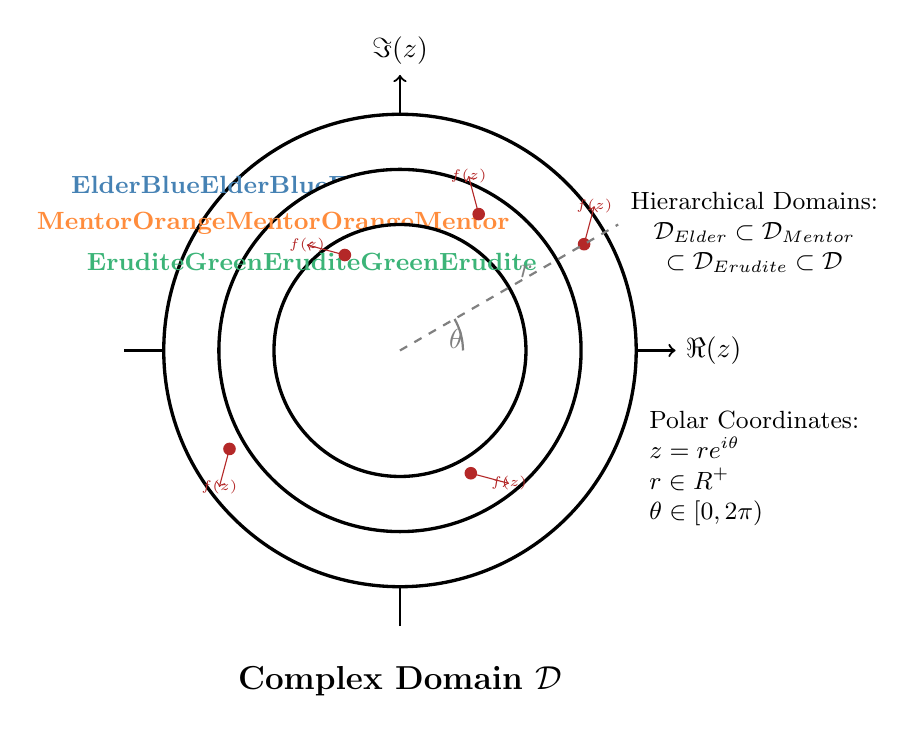
\begin{tikzpicture}[scale=1.0, every node/.style={transform shape}]

% Define colors matching Elder theme
\definecolor{ElderBlue}{RGB}{70, 130, 180}
\definecolor{MentorOrange}{RGB}{255, 140, 60}
\definecolor{EruditeGreen}{RGB}{60, 180, 120}
\definecolor{DeepRed}{RGB}{180, 40, 40}

% Complex plane axes
\draw[black, thick, ->] (-3.5, 0) -- (3.5, 0) node[right] {$\Re(z)$};
\draw[black, thick, ->] (0, -3.5) -- (0, 3.5) node[above] {$\Im(z)$};

% Annular regions representing gravitational strata
\foreach \r/\color/\alpha/\label in {3/ElderBlue/0.15/Elder, 2.3/MentorOrange/0.15/Mentor, 1.6/EruditeGreen/0.15/Erudite} {
    \draw[\color, very thick, fill=\color!\alpha] (0,0) circle (\r);
    \node[\color, font=\small\bfseries] at ({-\r*0.7}, {\r*0.7}) {\label};
}

% Sample points showing heliomorphic function values
\foreach \angle/\r in {30/2.7, 60/2.0, 120/1.4, 210/2.5, 300/1.8} {
    \coordinate (P) at (\angle:\r);
    \fill[DeepRed] (P) circle (0.08);
    \draw[DeepRed, ->] (P) -- +(\angle+45:0.5) node[font=\tiny] {$f(z)$};
}

% Radial and angular coordinates
\draw[dashed, gray, thick] (0,0) -- (30:3.2);
\draw[gray, thick] (0.8,0) arc (0:30:0.8);
\node[gray, right] at (0.5,0.15) {$\theta$};
\node[gray, above] at (1.6,0.8) {$r$};

% Domain labels
\node[black, font=\large\bfseries] at (0, -4.2) {Complex Domain $\mathcal{D}$};

% Hierarchical domain relationships
\node[black, font=\small, align=center] at (4.5, 1.5) {
    Hierarchical Domains:\\
    $\mathcal{D}_{\text{Elder}} \subset \mathcal{D}_{\text{Mentor}}$\\
    $\subset \mathcal{D}_{\text{Erudite}} \subset \mathcal{D}$
};

% Coordinate system explanation
\node[black, font=\small, align=left] at (4.5, -1.5) {
    Polar Coordinates:\\
    $z = re^{i\theta}$\\
    $r \in \mathbb{R}^+$\\
    $\theta \in [0, 2\pi)$
};

\end{tikzpicture}

\caption{Complex Domain Structure for Heliomorphic Functions. The domain $\mathcal{D}$ is stratified into hierarchical annular regions corresponding to Elder, Mentor, and Erudite subspaces. Each region has distinct gravitational field properties that influence the behavior of heliomorphic functions. Sample function values $f(z)$ are shown at various points, demonstrating the polar coordinate system $(r, \theta)$ used throughout the Elder Theory framework.}
\label{fig:heliomorphic_domain}
\end{figure}